\chapter{Sperimentazione}
\label{chap:lab}

% https://ntnuopen.ntnu.no/ntnu-xmlui/bitstream/handle/11250/2634012/no.ntnu:inspera:2440645.pdf

Dopo tante parole spese, è il momento giusto per soffermarsi a ricapitolare. Finora abbiamo visto le nozioni principali ed il percorso storico che hanno accompagnato lo sviluppo delle reti Internet, culminati nell'architettura ETSI NFV. Abbiamo parlato del software atto a realizzare un router interamente virtuale e delle ottimizzazioni necessarie affinché sia il più efficiente possibile, motivando ogni scelta. Infine, abbiamo accennato come questo software possa essere inserito in un più complesso sistema di orchestrazione, citando alcuni esempi.

Ora bisogna passare dalla teoria alla pratica. Questo capitolo tratta il nostro tentativo di deployare un router completamente virtuale sopra un hypervisor. In particolare, racconteremo le sfide, i problemi, le soluzioni e gli interrogativi ancora aperti. L'obiettivo è sperimentare quanto visto con VPP/DPDK e KVM, utilizzando TNSR come base di partenza. Non affronteremo il tema dell'orchestrazione e dell'automazione, scelta necessaria dato il tempo a disposizione.

\section{Hardware}

Conditio sine qua non per poter effettuare degli esperimenti è disporre di un laboratorio. La culla dove realizzarlo è stato il TOP-IX, l'Internet Exchange di Torino, che ha messo a disposizione hardware e conoscenze fondamentali. Nello specifico, abbiamo usato:

\begin{itemize}
    \item 2 server Supermicro SYS-1029U-TRTP2 (\textit{hyper1} e \textit{hyper2}) adibiti a virtualizzatori, ciascuno con a bordo 2 processori Intel Xeon Silver 4210R e 128 GB di RAM in configurazione a 3 canali. Inoltre, abbiamo montato le seguenti schede di rete aggiuntive:
    \begin{itemize}
        \item hyper1, Mellanox ConnectX-4 Lx CX4121A-XCAT con due interfacce a 10 Gbps
        \item hyper2, Intel X710-BM2 con due interfacce a 10 Gbps e Intel E810-CAM2 con due interfacce a 100 Gbps
    \end{itemize}
    \item 1 server Supermicro SYS-1029U-TRTP2 con 2 processori Intel Xeon Silver 4210R e 384 GB di RAM in configurazione a 3 canali, usato come traffic generator (\mbox{\textit{tg-monster}}), a cui è stata aggiunta una scheda Intel XXV710 con due interfacce a 25 Gbps
    \item 1 switch Nokia 7250 IXR-e Big 2QSFP28 8SFP28 24SFP+, centro stella della nostra rete
    \item 1 router Mikrotik CCR1036-8G-2S+ usato come traffic generator
    \item 1 switch Mikrotik CRS317-1G-16S+ usato come switch di supporto
\end{itemize}

Su tutti e tre i server abbiamo installato Ubuntu Server 20.04 LTS. Per hyper1 e hyper2 abbiamo aggiunto due parametri alla command line di Linux affinché il passthrough dei device PCIe avvenisse senza problemi:

\begin{figure}[h!]
\centering
\begin{BVerbatim}
GRUB_CMDLINE_LINUX_DEFAULT="intel_iommu=on iommu=pt"
\end{BVerbatim}
% \caption{C++ code}
\end{figure}

Quest'accortezza serve a istruire il sistema operativo su come inizializzare le \mbox{IOMMU}, l'equivalente delle MMU per i device PCI, permettendo ai dispositivi di accedere direttamente alla memoria (DMA) delle VM come se fossero bare metal.

Per la gestione delle macchine virtuali abbiamo usato \textit{virt-manager}, un front-end grafico di \textit{libvirt} che ha la funzione di interfacciarsi con svariati virtualization engines (tra cui KVM) ed astrarne il funzionamento.

A livello topologico ci sono due reti: la prima, quella di test, isolata dal resto, vede al centro lo switch Nokia con attorno collegati tutti i dispositivi. Sullo switch sono configurati due broadcast domain che raggruppano le interfacce: le porte pari in uno, le dispari nell'altro. 

Come da prassi consolidata, è poi presente una seconda rete, raccolta da un classico switch Ethernet, dedicata al management via SSH ed accessibile via VPN. In questa rete ciascuna VM dispone di un'interfaccia collegata ad un bridge virtuale connesso ad una porta fisica dedicata dell'hypervisor, il quale è a sua volta attestato sulla stessa rete in maniera indipendente tramite altre due porte LAN: su una è in ascolto il server SSH del sistema operativo, l'altra invece è gestita da IPMI, un management avanzato che permette di avere controllo dell'intero hardware da remoto.

\begin{figure}[htb]
    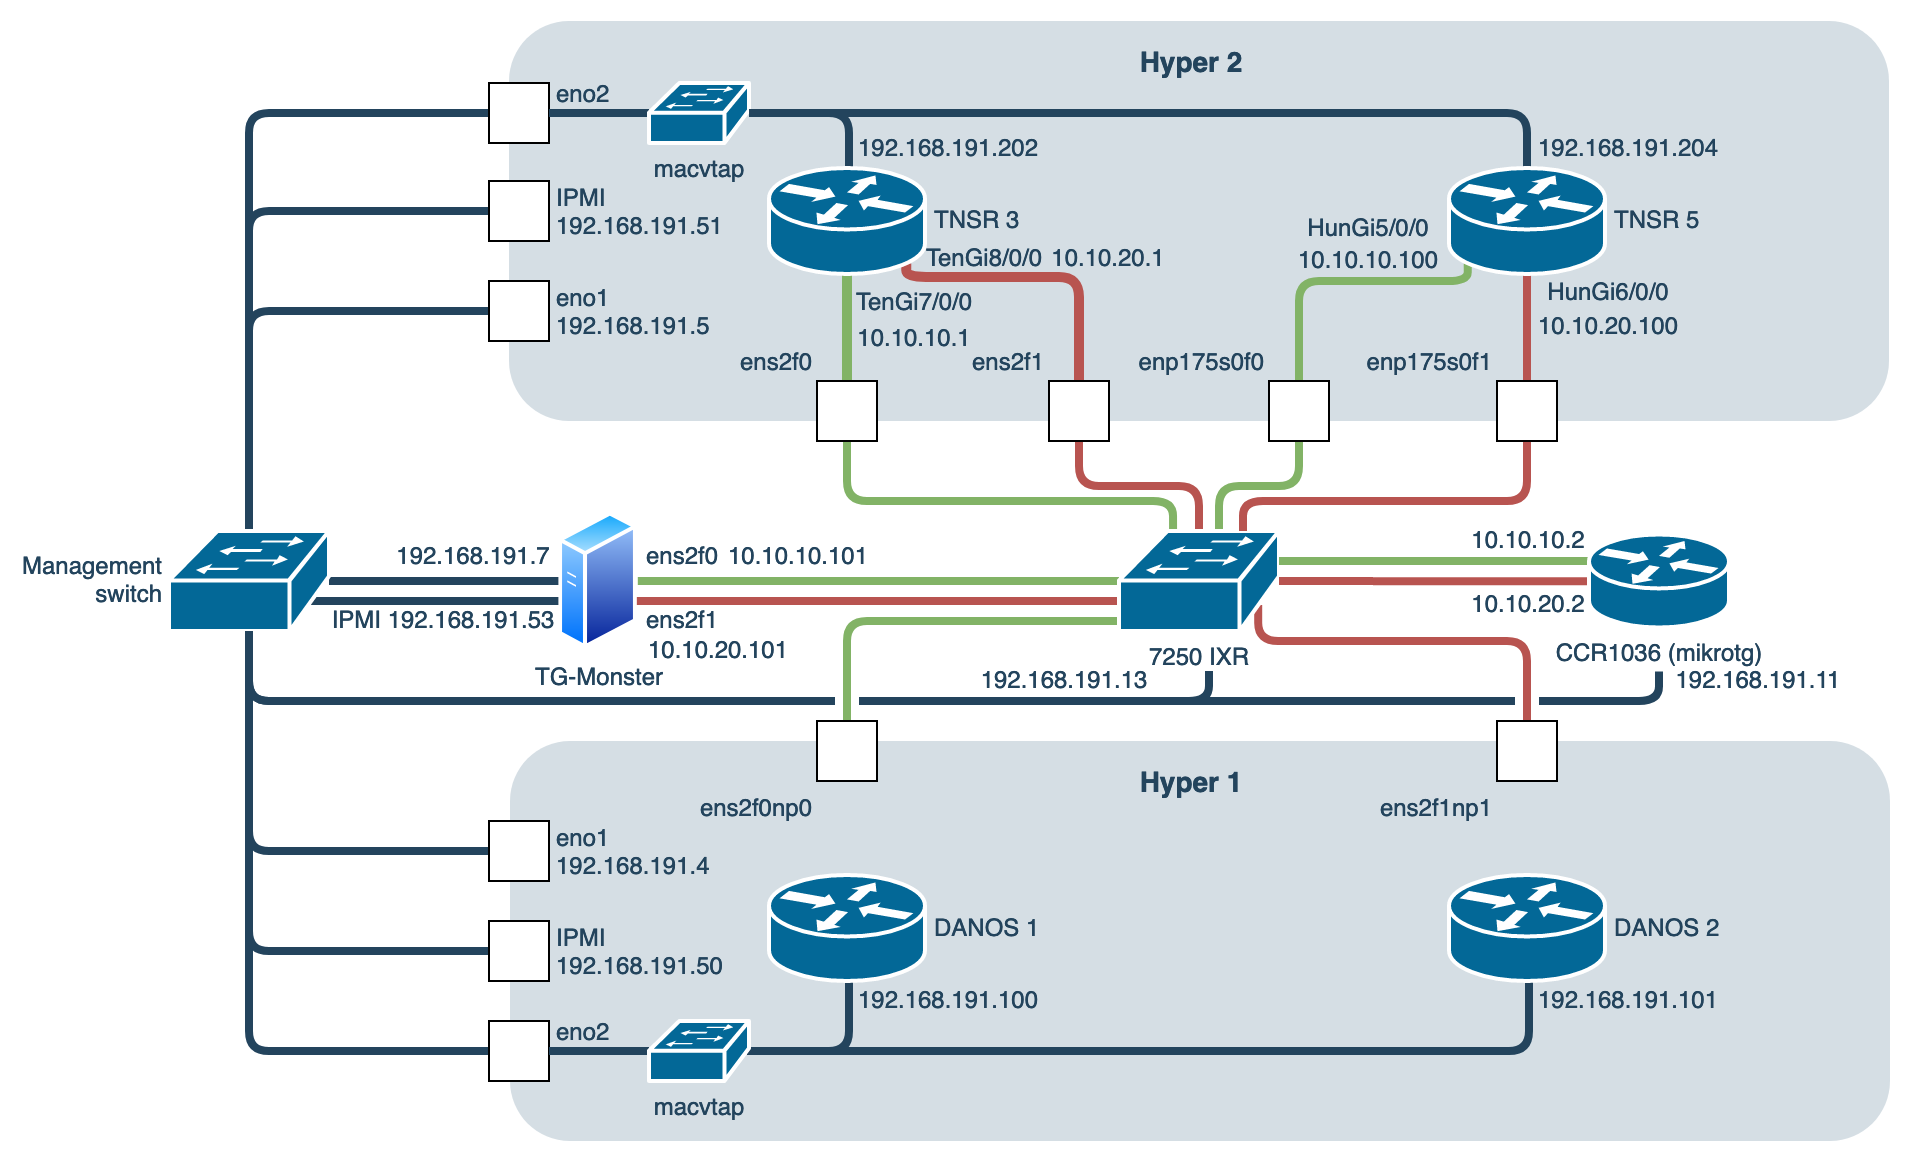
\includegraphics[width=0.8\textwidth]{graphics/vlan-191.png}
    \caption{Schema di rete del laboratorio}
    \label{fig:vlan-191}
\end{figure}

\section{Primi test}

Innanzitutto abbiamo provato a vedere se fosse possibile instaurare una sessione BGP tra pochi router, scambiandosi dei prefissi. La topologia base era costituita da tre router: R1 al centro, R2 ed R3 ai bordi, ciascuno su un sistema autonomo distinto. R1 simulava un route reflector e ridistribuiva i prefissi imparati via eBGP, R2 ed R3 possedevano ciascuno una LAN in classe C connessa e la annunciavano. Ogni router era identificato dall'indirizzo di loopback assegnato ad un'interfaccia dedicata. Le punto-a-punto erano realizzate semplicemente con un bridge virtuale nell'hypervisor.

\begin{figure}[htb]
    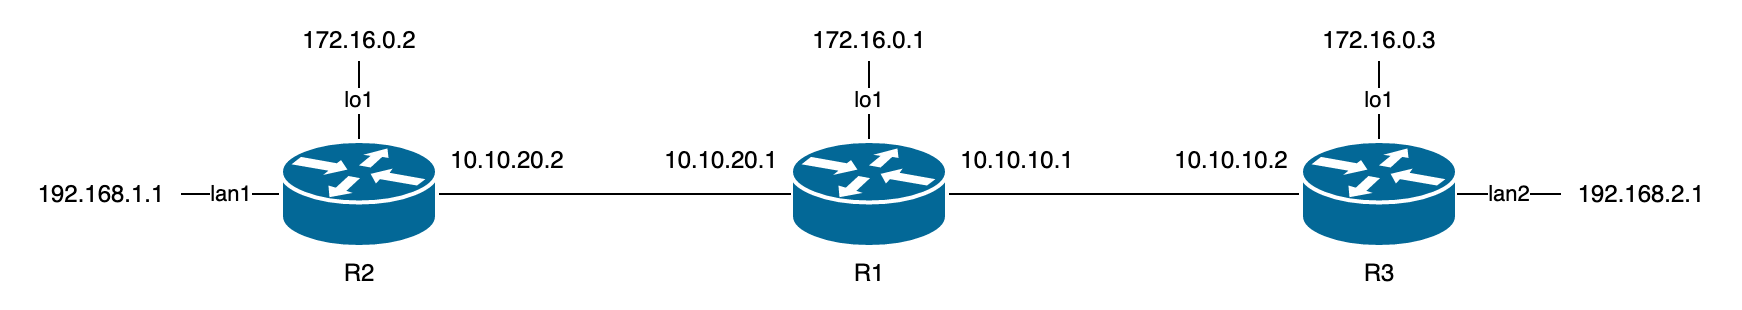
\includegraphics[width=0.8\textwidth]{graphics/bgp-topo-1.png}
    \caption{Topologia iniziale}
    \label{fig:bgp-topo-1}
\end{figure}

La rete funzionava ed era possibile contattare l'interfaccia \textit{lan2} di R3 dalla \textit{lan1} di R2, verificando nel traceroute che si passasse effettivamente per R1. Dapprima abbiamo usato TNSR su ciascun router, poi abbiamo provato a sostituirne alcuni con DANOS o VyOS, verificando il corretto funzionamento ogni volta. Ciò è stato utile per provare che non solo i diversi control plane funzionassero, ma che fosse anche possibile interconnettersi ad altri apparati tramite protocolli standard.

\section{SMT}

\textit{Simultaneous Multi-Threading} (SMT) è una tecnologia che consente a due o più thread applicativi di essere eseguiti contemporaneamente su uno stesso core fisico. Un moderno microprocessore dispone di abbondanti capacità di memorizzazione ed elaborazione, difficili da sfruttare appieno con il solo \textit{Instruction Level Parallelism} (ILP). Con SMT le risorse vengono partizionate dinamicamente e ripartite tra i thread con pochissimo overhead, poiché si può fare affidamento a tutto lo scheletro già presente per l'esecuzione multiple issue di ILP, apportando piccole modifiche.

Nel paragrafo \ref{sec:vpp} abbiamo visto come VPP sfrutti il processing vettoriale per aumentare il throughput, elaborando grandi insiemi di dati alla volta piuttosto che singolarmente. SMT d'altra parte, dividendo le risorse tra più thread, ottiene l'effetto contrario: ogni thread che operi a pieno regime potrà sfruttare solo metà delle \eng{instruction} cache e data cache disponibili nel core, intaccando sensibilmente le performance di VPP.

\begin{figure}[htb]
    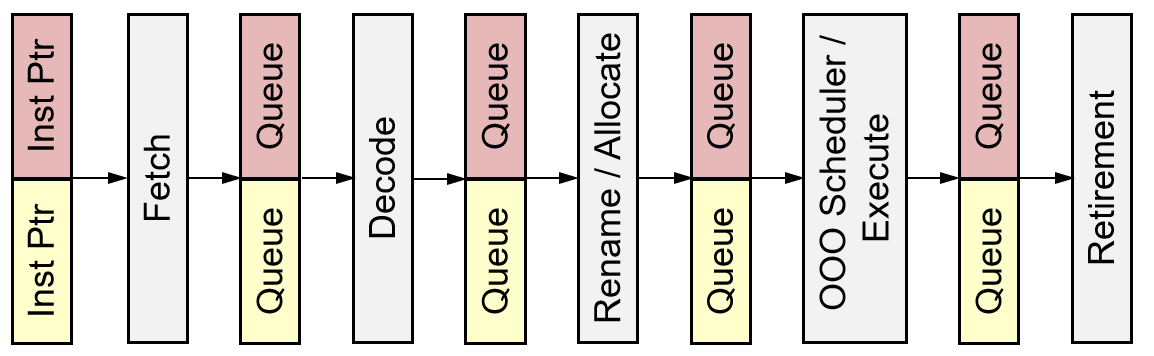
\includegraphics[width=0.7\textwidth]{graphics/smt.png}
    \caption{Ripartizione delle instruction queue in SMT}
    \label{fig:smt}
\end{figure}

Alcuni semplici test effettuati in locale hanno confermato quanto da molti riportato online: SMT, commercializzato da Intel col nome \textit{``Hyper-Threading''}, rallenta VPP, motivo per il quale abbiamo deciso di disabilitarlo fin da subito.

\section{Traffic generation}

% Appurato che il peering funzionasse, abbiamo staccato i due router laterali e mappato le porte di R1 sulle interfacce fisiche dell'hypervisor (PCI passthrough). Queste erano collegate al CRS317 al quale era connesso pure il CCR1036. Il Mikrotik, da specifica, è in grado di generare traffico a 10 Gbps verso destinazioni configurabili, adeguato al nostro obiettivo di raggiungere il \textit{line rate} escludendo dal test variabili legate al generatore.

A valle del controllo di configurazione BGP, abbiamo proceduto a verificare le prestazioni del singolo router. La macchina R1 ha visto le proprie interfacce mappate su quelle fisiche dell'hypervisor in PCI passthrough. A questo punto abbiamo utilizzato il router CCR1036 per generare diversi pattern di traffico passanti per R1. Il Mikrotik è stato scelto in quanto permette di generare flussi di 10 Gbps line rate su singola interfaccia in modalità stateless, valore adeguato al nostro obiettivo di test.

``Line rate'' è un termine che si riferisce alla capacità di un apparato di raggiungere e mantenere una certa velocità operativa indipendentemente dalla dimensione dei pacchetti dati. Come riferimento, si usa un pacchetto L2 da 64 byte (60 di payload + 4 di frame check sequence) a cui, nel caso di Ethernet, vanno aggiunti 8 byte di preambolo, 1 byte di epilogo e 11 byte di inter-frame gap, portando la dimensione totale a 84 byte. A questo punto è facile calcolare il packet-rate corrispondente a 10 Gbps:

\begin{equation} \label{eq:10g-line-rate}
    \frac{10\ Gbps}{84\ byte \cdot 8} \approx 14.88\ Mpps
\end{equation}

Il primo test ``a scatola chiusa'' ha mostrato che DANOS era in grado di raggiungere circa 11 Mpps nel puro forwarding IP tra due interfacce, mentre TNSR si fermava a metà: 5.5 Mpps. A questo punto le basi teoriche esposte nel \cref{chap:software} non erano ancora ben consolidate ed abbiamo cercato di indagare per scoprire la ragione di questi risultati, incuriositi dal fatto che uno fosse esattamente il doppio più veloce dell'altro.

\section{Receive Side Scaling}

Nessun microprocessore, per quanto potente, è in grado di scalare all'infinito accomodando moli sempre più crescenti di traffico. Occorre un metodo per suddividere il carico tra molteplici worker in maniera che possa essere gestito in parallelo. Il modo più intuitivo consisterebbe nel definire $n$ code in ricezione (\textit{receive queues} o \mbox{\textit{rx-queues}}) e ripartire i pacchetti tra esse secondo un algoritmo round-robin. Tuttavia un'equa spartizione di questo tipo avrebbe il probabile effetto di trattare diversamente pacchetti di uno stesso flusso end-to-end, generando imprevedibilità nella rete: i dati potrebbero giungere a destinazione seguendo strade diverse e con diverse latenze, andando direttamente a pesare su quei trasporti come TCP che devono riordinare i dati prima di consegnarli al livello applicativo, oppure perdersi in parte. Per questo motivo al round-robin tradizionale si preferisce una soluzione equivalente che cerchi di preservare ogni flusso nella sua interezza.

Receive Side Scaling (RSS) è l'approccio proposto da Microsoft e largamente adottato: un classificatore hardware ridistribuisce i pacchetti su un numero configurabile di code basandosi su un hash\footnote{\ Algoritmo proprietario calcolato dalla NIC stessa e diverso per ciascun produttore} degli indirizzi sorgente e destinazione di livello 3 e 4, oppure sulle etichette MPLS, assumendo così un significato semantico analogo alla flow label di IPv6.

\begin{figure}[htb]
    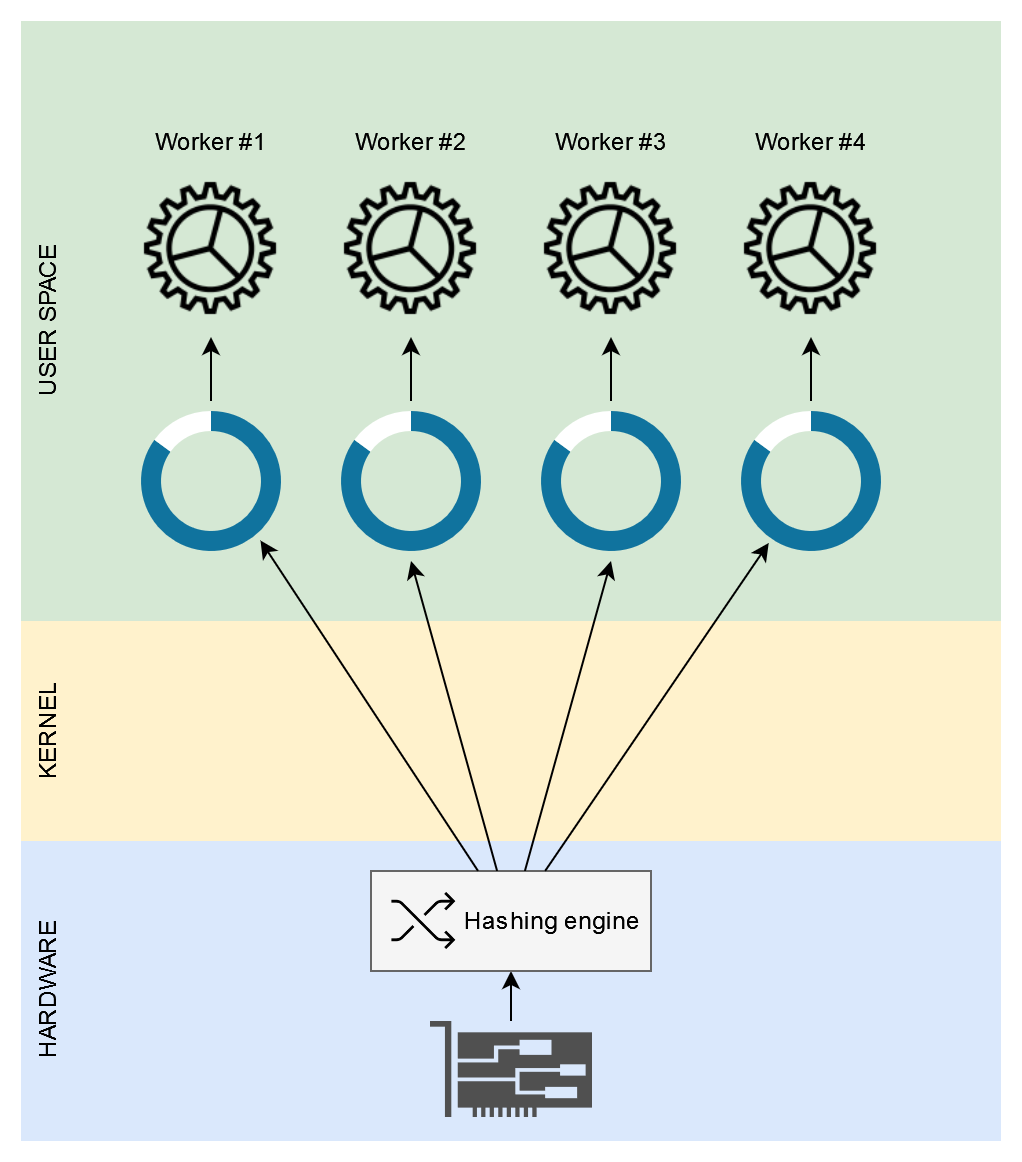
\includegraphics[width=0.7\textwidth]{graphics/rss.png}
    \caption{Receive Side Scaling\protect\footnotemark}
    \label{fig:rss}
\end{figure}
\footnotetext{\ I buffer sono rappresentati in user space, forma ottenibile con l'ausilio di DPDK}

Un criterio affine è adottato in ambiti diversi, come il load balancing: nel definire un \textit{link aggregation} (LAG) i vendor adottano un sistema simile per ripartire il traffico basandosi su hashing. Le NIC moderne, come la Intel E810 da noi testata, consentono di andare oltre e sostituire il classificatore con un microprogramma personalizzato. Questo apre ad un'infinità di possibilità come differenziare il traffico in base alla sua natura: un operatore mobile potrebbe voler dare priorità ai flussi LTE Voce a discapito dei pacchetti dati, assegnando ai primi delle code pregiate con worker dedicati e rilegando gli altri a buffer best effort con le risorse rimanenti.

Quanto appreso con RSS ci ha permesso di capire che DANOS stava adoperando dietro le quinte 2 rx-queues con altrettanti worker dedicati. TNSR invece di default ne usava una sola, ma a differenza di DANOS permetteva di modificare questo parametro. Alzando le rx-queues a 2 abbiamo ottenuto prestazioni in linea con DANOS. La vera sorpresa però è stata quando abbiamo ulteriormente aumentato fino a 4 code: i risultati erano identici. In seguito alla verifica inconcludente di molteplici configurazioni, abbiamo provato a replicare l'esperimento su hyper2 sfruttando la scheda Intel che fin da subito ha raggiunto il line rate.
% L'ipotesi più accreditata è che l'RSS della Mellanox non riuscisse a ripartire correttamente i flussi del Mikrotik su più code, essendo questi sostanzialmente identici end-to-end.
Pur non disponendo una prova formale, supponiamo che la funzione di hashing della modalità RSS implementata nella NIC Mellanox non riuscisse a ripartire correttamente su più code il traffico di test, probabilmente per mancanza di entropia negli \textit{headers} dei pacchetti utilizzati al fine del bilanciamento.
La Intel verosimilmente implementa un algoritmo di hashing diverso, in grado di distribuire equamente il traffico anche in casi come questo. Onde evitare il ripetersi dell'anomalia, si è deciso di cambiare traffic generator, installando TRex su \mbox{tg-monster} cosicché si potesse trarre vantaggio dalla maggiore entropia dei flussi.

\section{NUMA pinning} % isolcpus

Raggiunto il traguardo dei 10 Gbps line rate, lo step successivo era verificare quanto potesse scalare. Il CRS317 è stato sostituito dal Nokia, equipaggiato di porte a 25 e 100 Gbps, al posto del CCR1036 abbiamo messo il server dedicato con TRex e su hyper2 abbiamo montato la scheda Intel E810. Questa riorganizzazione era anche un buon momento per ottimizzare il layout fisico delle macchine virtuali: nel \cref{chap:virt} si è discusso di come un deploy NUMA-aware sia imprescindibile per raggiungere target di un certo calibro. A tal proposito, KVM permette di esplicitare i core fisici sui cui mappare i thread virtuali delle VM tramite l'attributo \verb|cpuset|.

\begin{figure}[htb]
    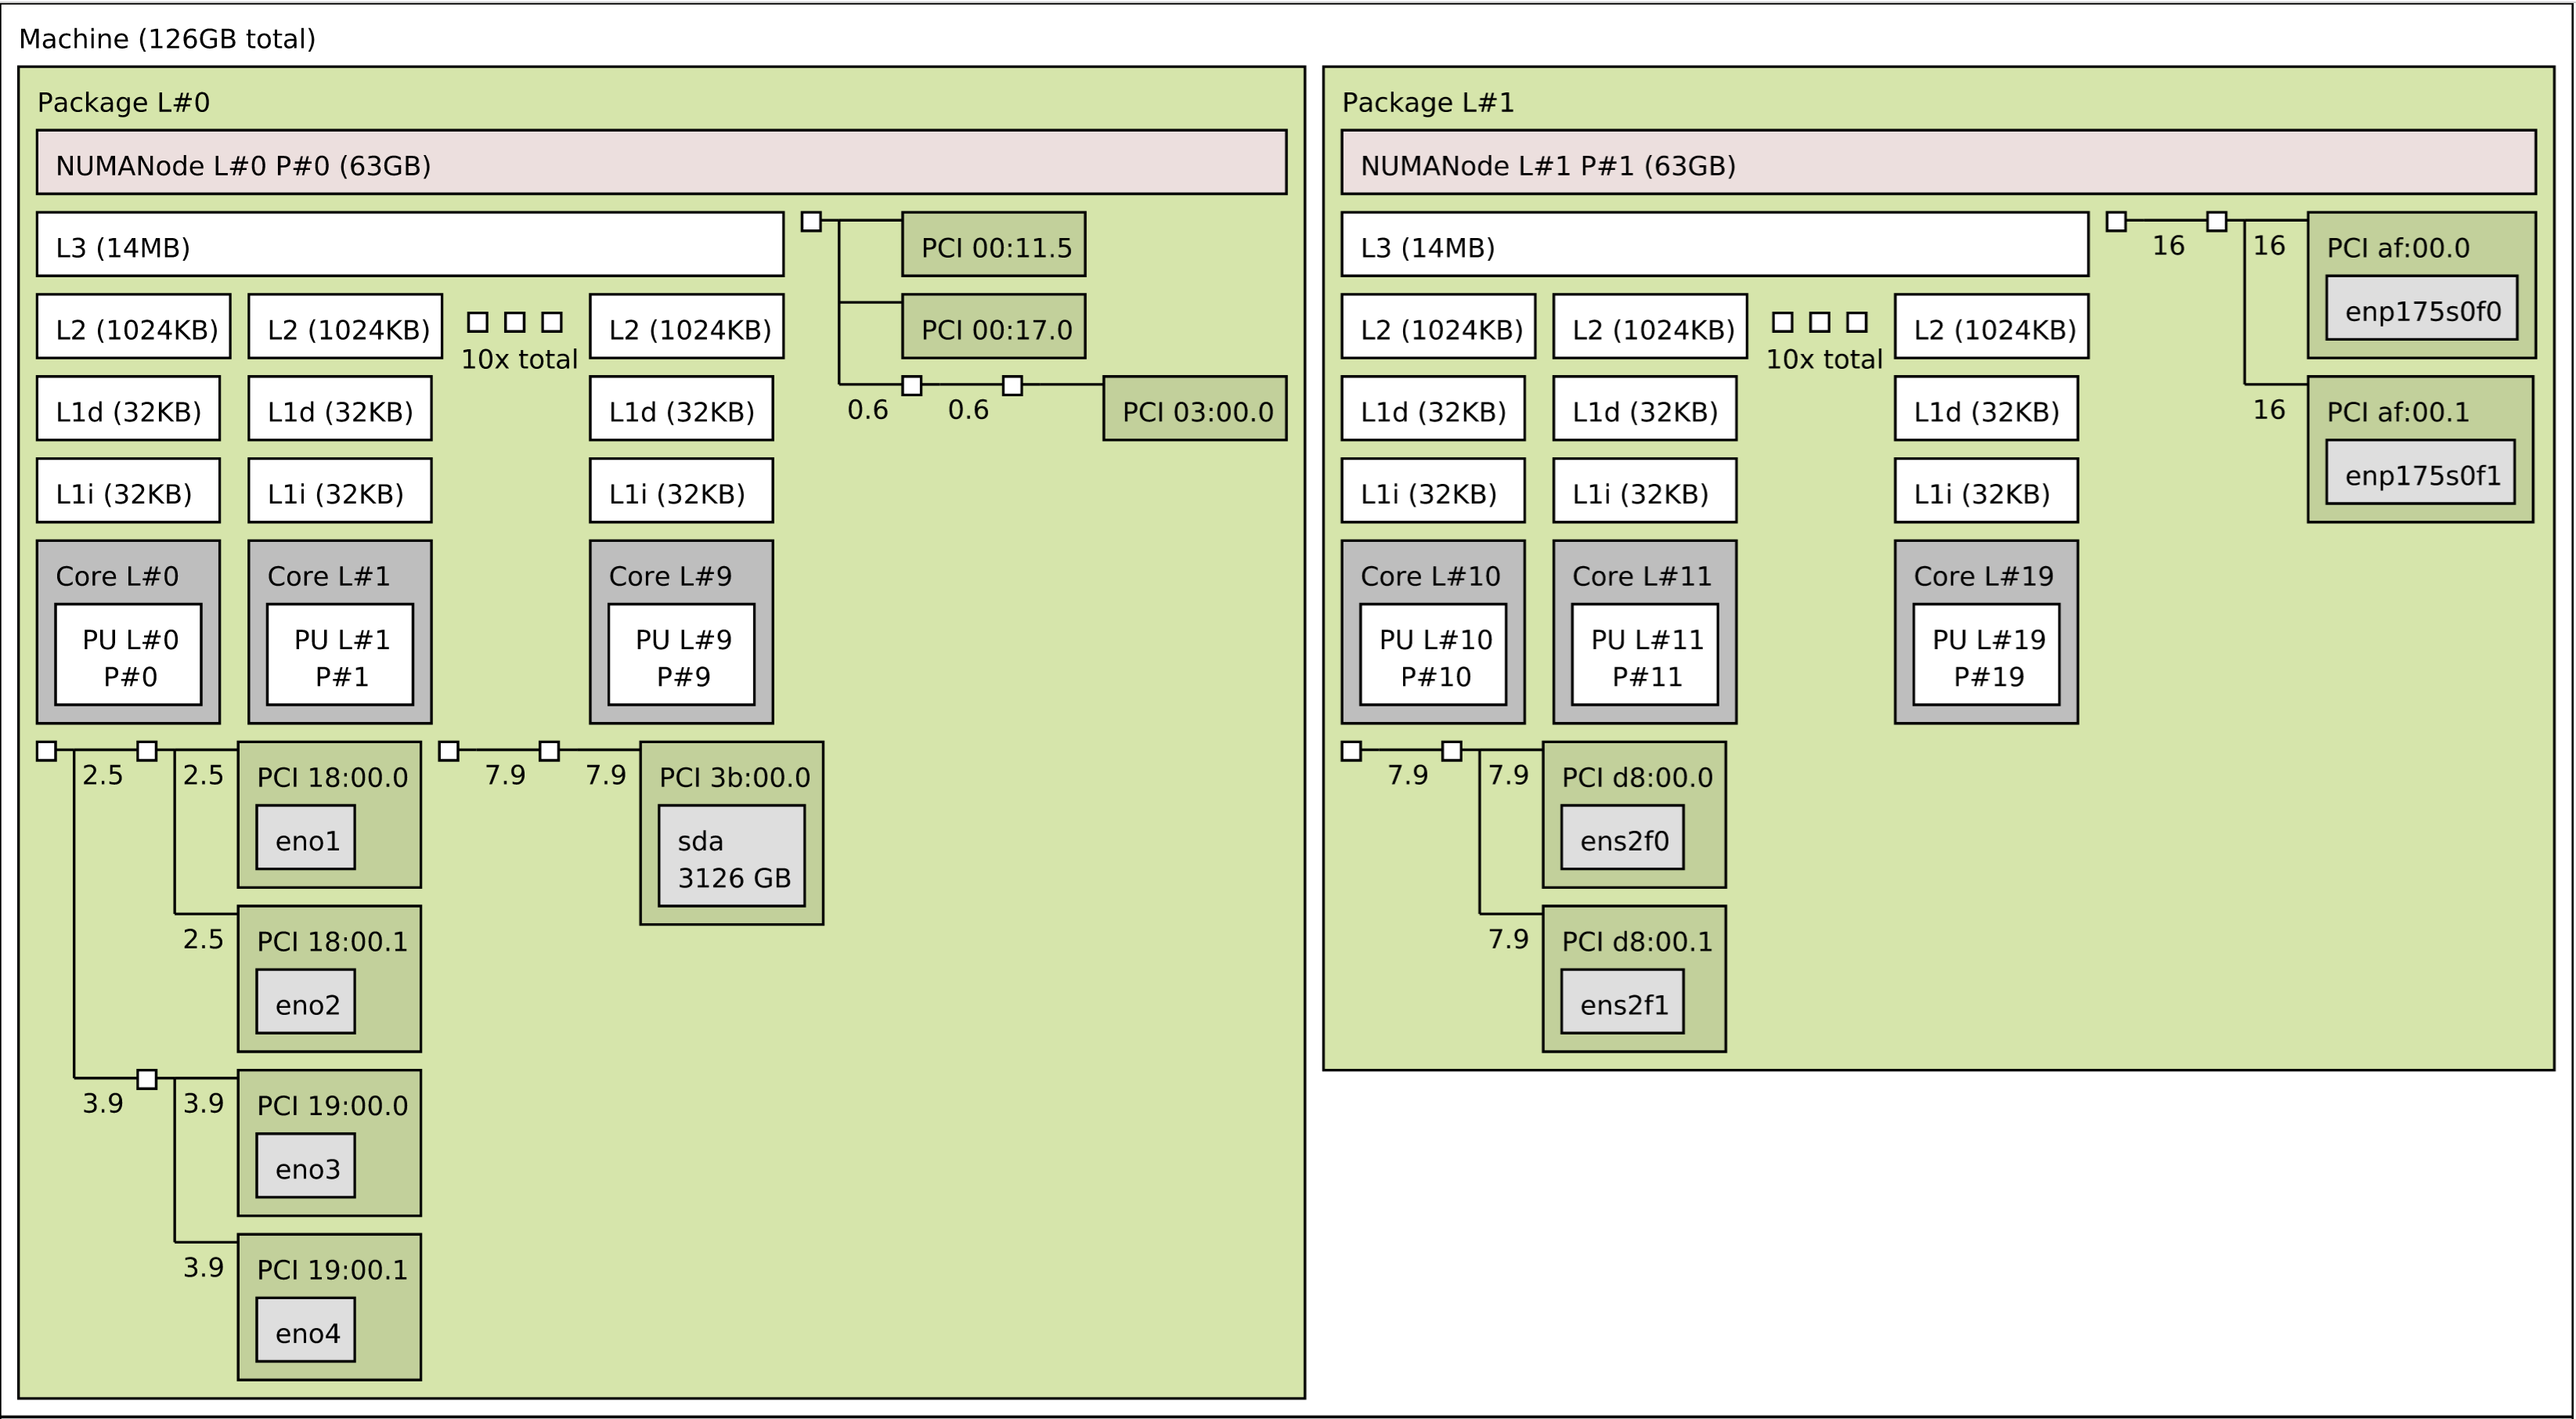
\includegraphics[width=0.8\textwidth]{graphics/hyper2topohd.png}
    \caption{Topologia fisica di hyper2}
    \label{fig:hyper2topo}
\end{figure}

In figura \ref{fig:hyper2topo} è rappresentata la topologia fisica di hyper2 ottenuta tramite lo strumento \verb|lstopo|. Si possono distinguere chiaramente i due nodi NUMA: del primo fanno parte \mbox{CPU0} (core da 0 a 9), \mbox{64 GB} di memoria, le 4 interfacce di rete integrate del server, lo storage (\textit{sda}) e altri dispositivi minori. Nel secondo invece troviamo CPU1 (core da 10 a 19), i restanti \mbox{64 GB} di RAM e le schede di rete aggiuntive: \textit{ens2} è la X710, mentre \textit{enp175s0} la E810; \textit{f0} ed \textit{f1} sono le due interfacce fisiche presenti su ciascuna NIC.

Per i test si è deciso di dedicare interamente CPU1 alla macchina virtuale con TNSR specificando l'attributo \verb|cpuset="10-19"| in KVM. Non solo, per evitare che quei core potessero essere usati dall'hypervisor per task di routine, li abbiamo esclusi dallo scheduling di Linux tramite il parametro \verb|isolcpus=10-19| alla cmdline del kernel. Così facendo la VM con TNSR ha assunto il controllo completo di CPU1 e dei device ad essa connessi, acquisiti con PCI passthrough. Volendo sarebbe stato possibile replicare una topologia NUMA verso la macchina virtuale, ma la poca familiarità con gli strumenti di virtualizzazione ci ha suggerito prudenza per non rischiare di compromettere i risultati sperimentali con errori grossolani dovuti all'inesperienza.

Il traffic generator prescelto, come anticipato, è stato TRex. Per il primo test abbiamo scelto un template IMIX da 1 Gbps, ossia un insieme di pacchetti di dimensione variabile rappresentativo di diverse tipologie di flussi dati: streaming, \eng{video conferencing}, navigazione web, mail, ecc. Il termine IMIX è infatti una sincrasi di ``Internet Mix'' per indicare la natura del traffico.

\begin{figure}[h!]
\centering
\begin{BVerbatim}
./t-rex-64 -f avl/sfr_delay_10_1g.yaml -m 25 -c 4 -l 1000
\end{BVerbatim}
% \caption{C++ code}
\end{figure}

Con questo comando abbiamo istruito TRex affinché generasse 25 Gbps di \eng{throughput} aggregato\footnote{\ Bidirezionale, circa 20 Gbps in una direzione e 5 Gbps nell'altra}: a partire da una base di 1 Gbps, questa andava amplificata 25 volte ed il test eseguito utilizzando 4 core del server.

\begin{figure}[htb]
    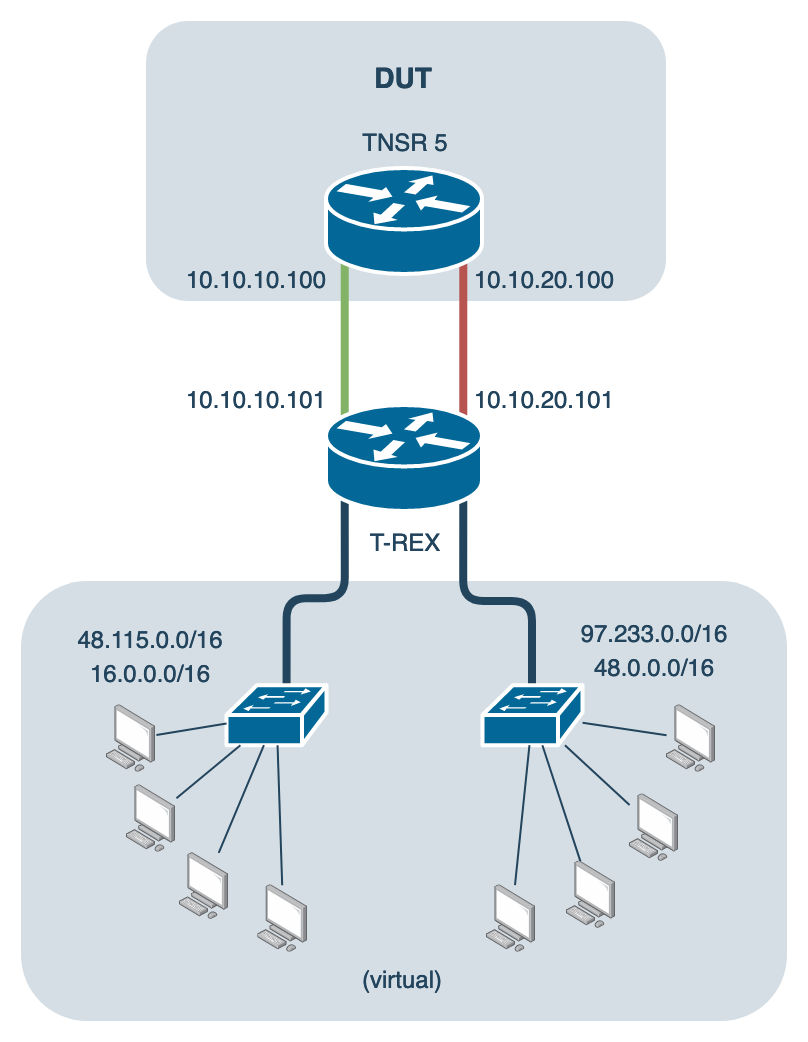
\includegraphics[width=0.5\textwidth]{graphics/trex-tnsr-dut.png}
    \caption{Schema del test}
    \label{fig:trex-tnsr-dut}
\end{figure}

I primi risultati sono stati soddisfacenti: 25 Gbps di traffico IMIX corrispondono ad appena 5.35 Mpps, entro il limite determinato sperimentalmente di un singolo core del nostro virtualizzatore. Quando però abbiamo provato ad aumentare il numero di worker per ripartire il carico, il router ha letteralmente smesso di funzionare: la quasi totalità dei pacchetti andava perduta o subiva latenze migliaia di volte più grandi di quelle misurate in precedenza. Dopo svariati tentativi andati a vuoto, non siamo riusciti a determinare la causa di questo problema, ma possiamo formulare delle ipotesi:

\begin{enumerate}
    \item TNSR viene fornito con la penultima versione di VPP e DPDK attualmente disponibili e noi, seguendo le indicazioni del manuale stesso di DPDK, abbiamo installato la penultima versione di driver e firware della scheda di rete. La prima ipotesi è dunque che si tratti di un bug, ma per verificarla occorrerebbe configurare da zero un'installazione di Linux con le ultime versioni di kernel, driver, VPP/DPDK e FRR.
    \item Tra le ottimizzazioni non prese in considerazione vi sono quelle legate alla memoria. In primis non abbiamo verificato che tutta la memoria riservata per la macchina virtuale risiedesse nel nodo NUMA in cui questa era collocata, fattore che però non avrebbe potuto a nostro avviso compromettere così gravemente le performance. In secondo luogo c'è il discorso \textit{hugepages}: come accennato nel paragrafo \ref{sec:dpdk}, DPDK fa uso di grandi aree di memoria contigua su cui mappare i buffer delle schede di rete. Linux permette di utilizzare 3 diverse dimensioni per le pagine di memoria: 4 KB (default), 2 MB e 1 GB, queste ultime definite ``huge pages''. Di default con KVM non è disponibile il supporto a pagine da 1 GB all'interno della VM: non sappiamo cosa succederebbe se il sistema operativo ospite provasse ugualmente ad allocarne, ma presumibilmente nulla di buono.
\end{enumerate}

La seconda ipotesi potrebbe essere avallata da un altro problema verificatosi in più occasioni: ogni volta che cercavamo di cambiare al volo il numero di code utilizzate dalla scheda di rete era necessario riavviare sia la macchina virtuale che l'hypervisor affinché queste modifiche avessero effetto. Questo comportamento è insolito e a riguardo possono esserci due spiegazioni:

\begin{enumerate}
    \item Riavviare il dispositivo, reinizializzandolo, provvede al reseeding dell'hashing engine di RSS che ha il compito di canalizzare il traffico sulle \mbox{rx-queues}. La nostra congettura è che questo non venga correttamente resettato quando si cambia dinamicamente il numero di code.
    \item Anche in questo caso il mapping tra memoria della macchina virtuale, memoria fisica e IOMMU potrebbe essere venuto meno, portando la NIC a scrivere i pacchetti ricevuti in aree di memoria non corrispondenti alle code allocate da DPDK.
\end{enumerate}

Tutti questi scenari sono difficili da investigare poiché richiedono grande dimestichezza con gli strumenti di diagnostica e una profonda conoscenza del funzionamento interno del software sottostante. Un aiuto potrebbe venire dall'indagare separatamente i problemi software da quelli legati all'infrastruttura di virtualizzazione, installando TNSR (o chi per esso) direttamente sul server fisico. Lo scopo di questa tesi però era indagare entrambi gli aspetti, motivo per il quale si era deciso di intraprendere la strada della virtualizzazione fin dall'inizio.

Purtroppo il tempo da dedicare a questa esperienza è terminato e gli interrogativi sopra esposti rimarranno aperti fino a quando qualcuno non si cimenterà nuovamente nell'impresa. Ammetto che non mi dispiacerebbe riprendere in mano questi argomenti un giorno, vedremo cosa ci riserverà il futuro.



% NUMA images
% https://cloudarchitectmusings.com/2012/12/17/the-impact-of-numa-on-virtualizing-business-critical-applications/
% https://frankdenneman.nl/2010/09/13/esx-4-1-numa-scheduling/ <<<===== CTO WMware